%!TEX root = ../thesis.tex

\section{Top Fan flips}

We never fan flip a fan flip again. We fan flip to remove large topfans. Say larger than 3.


We flip top fans from last fence upwards. We flip any topfan of 3 edges or larger.

Our flip differs slightly if we encounter a split in the bottom boundary path or a already flipped edge below on the rightmost bottom.

Refer to Figure \ref{fig:fanflip:fanflips} for the different kinds of topfanflips.


\begin{figure}
    \centering
    \begin{subfigure}[b]{0.8 \textwidth}
        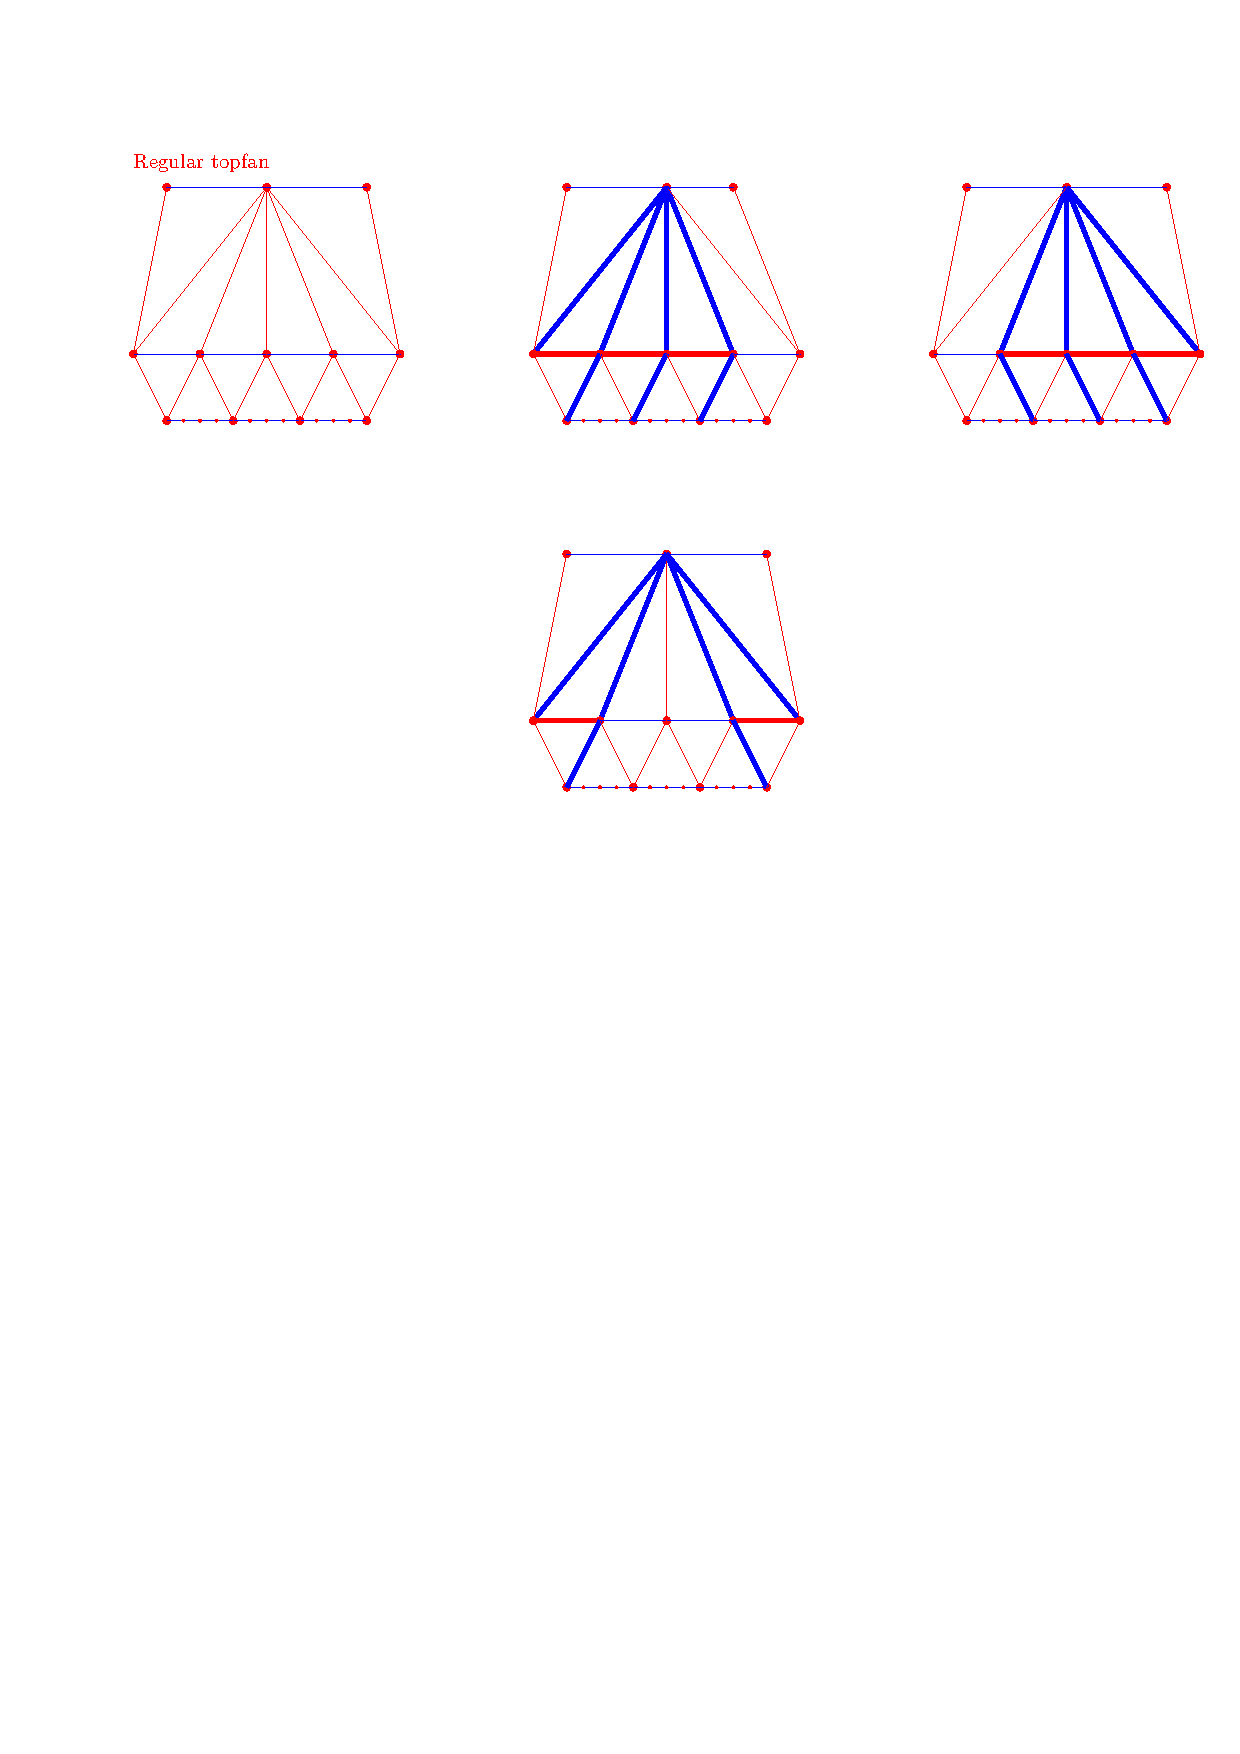
\includegraphics[width = \textwidth]{topFanFlips/img/regular}
        \caption{The regular topfanflip}
        \label{fig:fanflip:regular}
    \end{subfigure}
    ~
    \centering
    \begin{subfigure}[b]{0.45 \textwidth}
        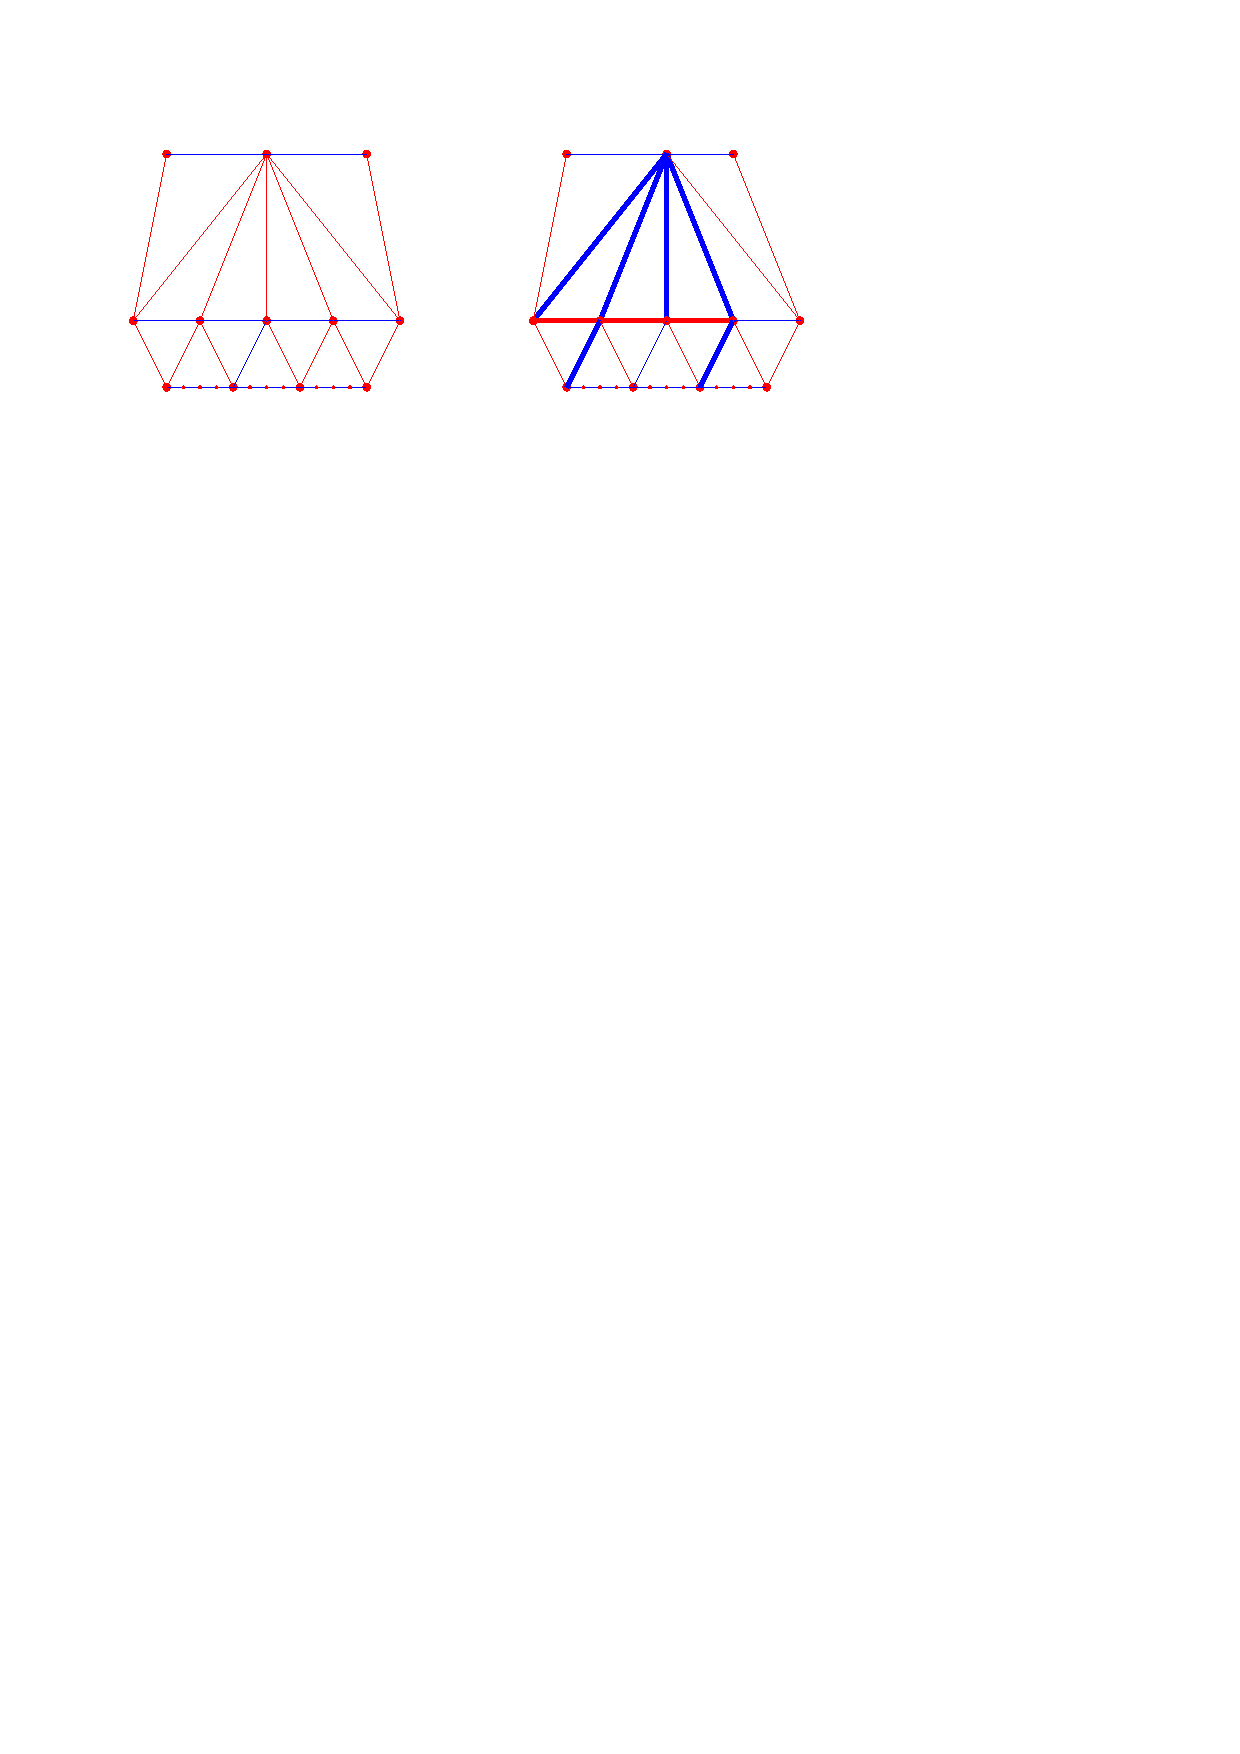
\includegraphics[width = \textwidth]{topFanFlips/img/merge}
        \caption{Topfanflip above a merge}
        \label{fig:fanflip:merge}

    \end{subfigure}
    ~
    \begin{subfigure}[b]{0.45 \textwidth}
        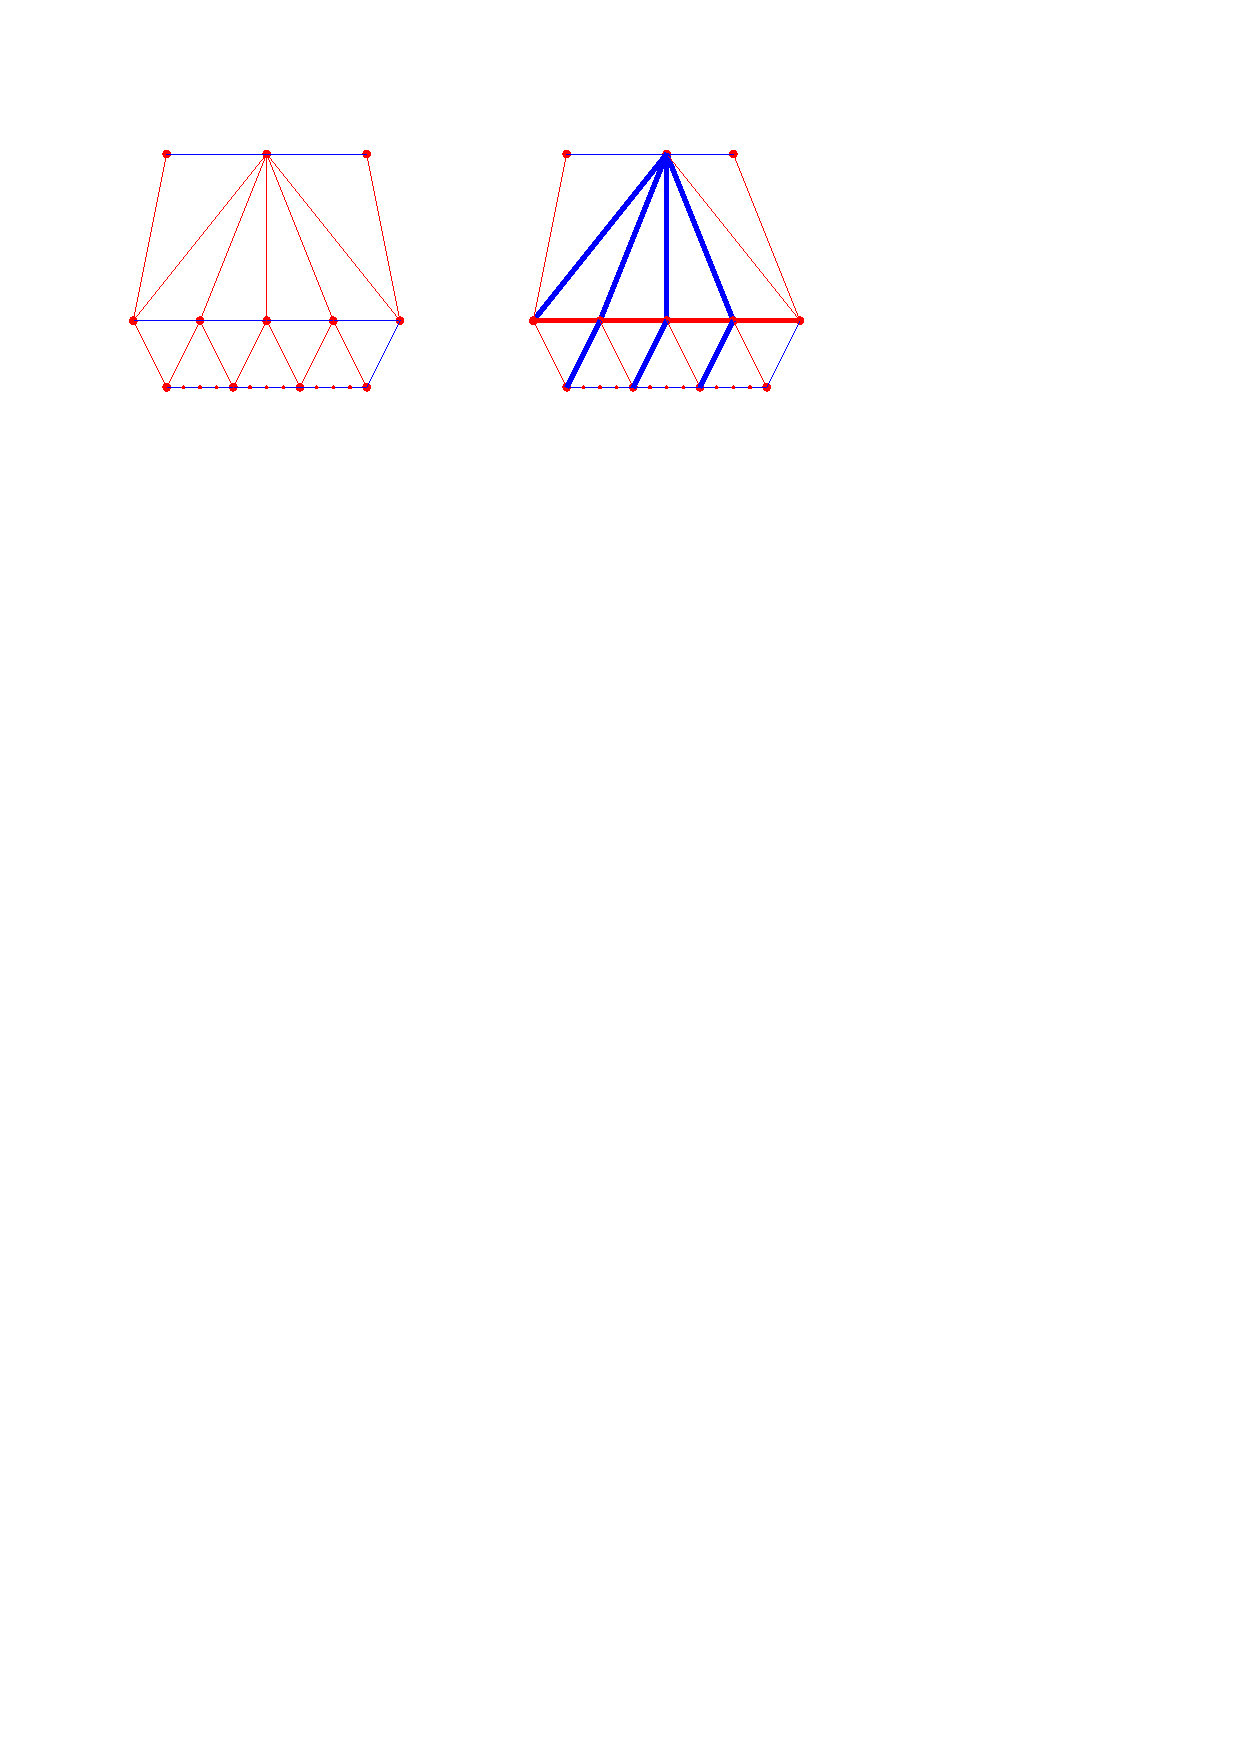
\includegraphics[width =\textwidth]{topFanFlips/img/mergeend}
        \caption{Topfanflip next to merge. Note the additional red edge.}
        \label{fig:fanflip:mergeLastVertex}

    \end{subfigure}
    \centering
    \begin{subfigure}[b]{0.45 \textwidth}
        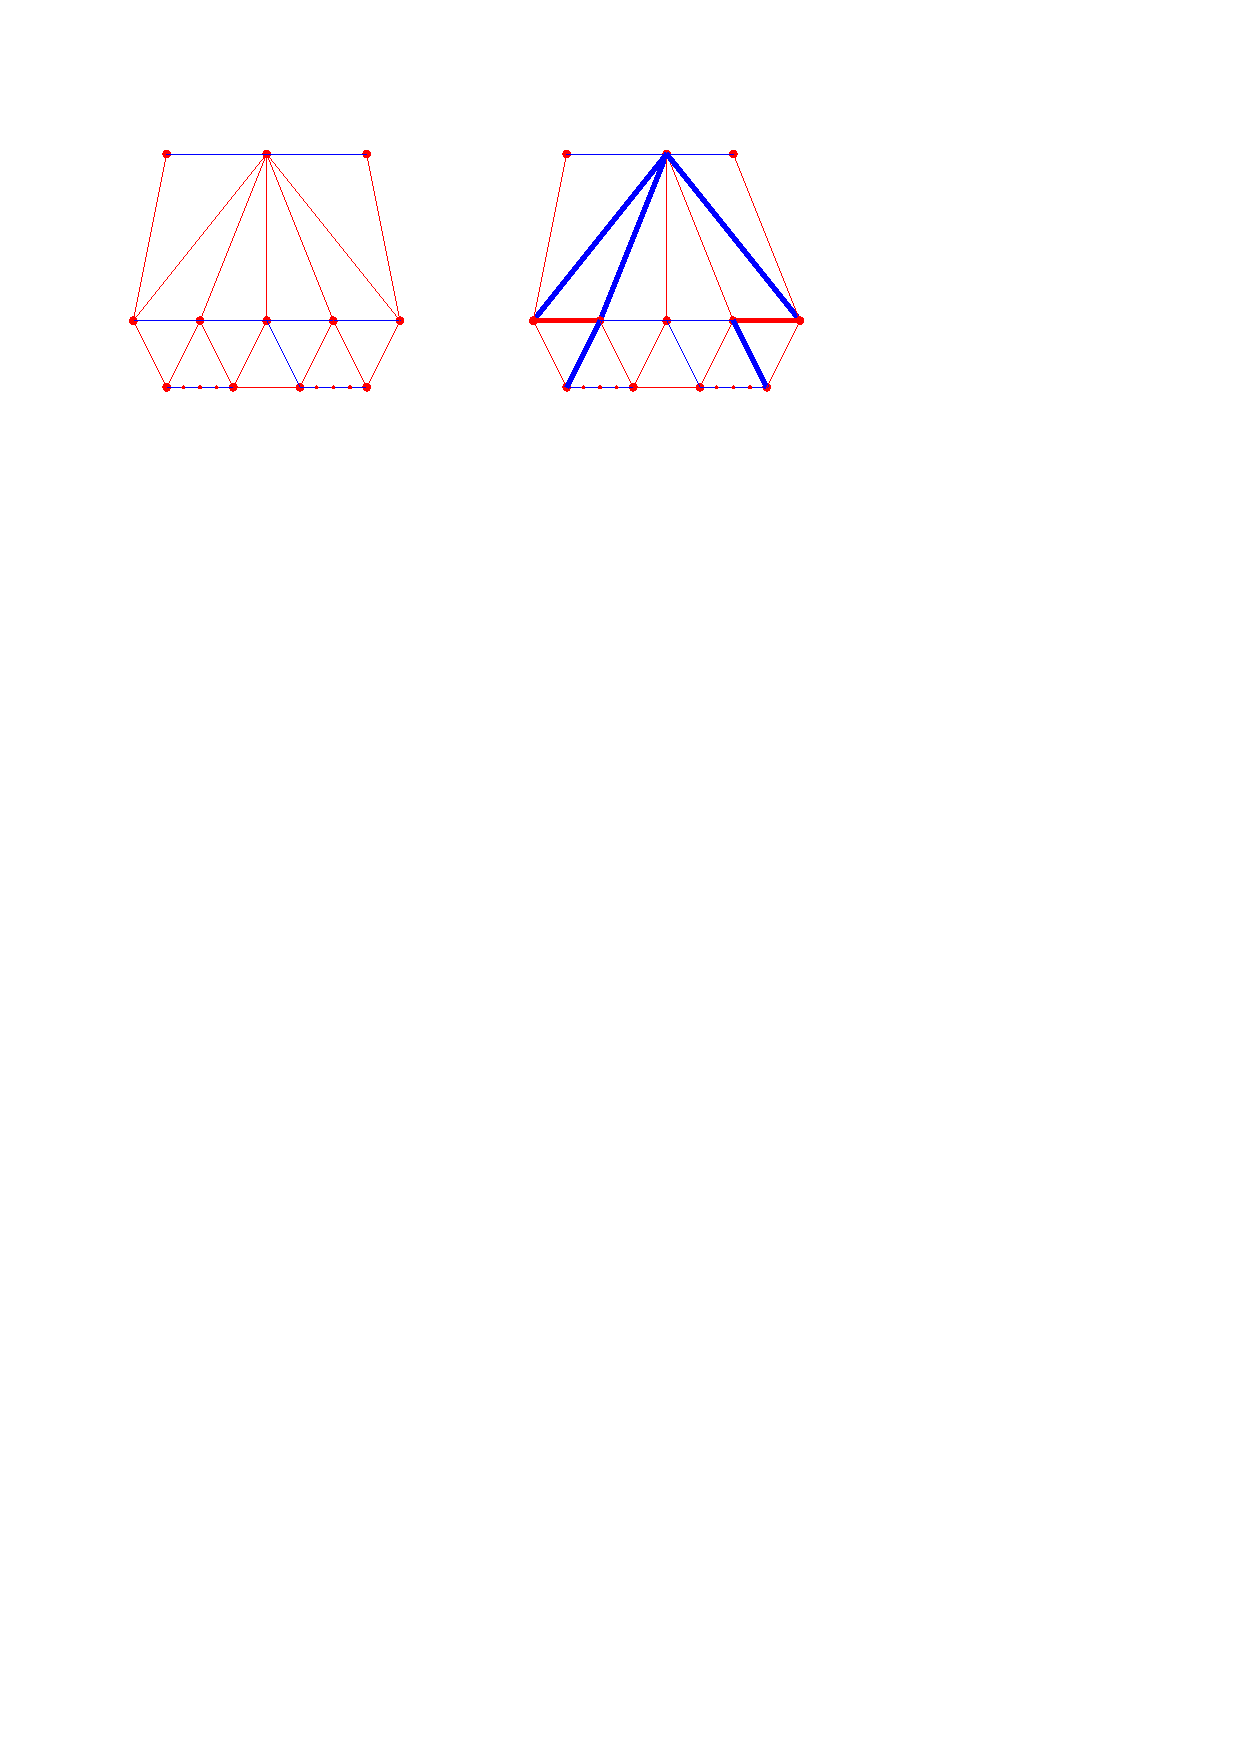
\includegraphics[width = \textwidth]{topFanFlips/img/split}
        \caption{Above a split we stop and we mark the last edge for topload}
        \label{fig:fanflip:split}

    \end{subfigure}
    ~
    \begin{subfigure}[b]{0.45 \textwidth}non
        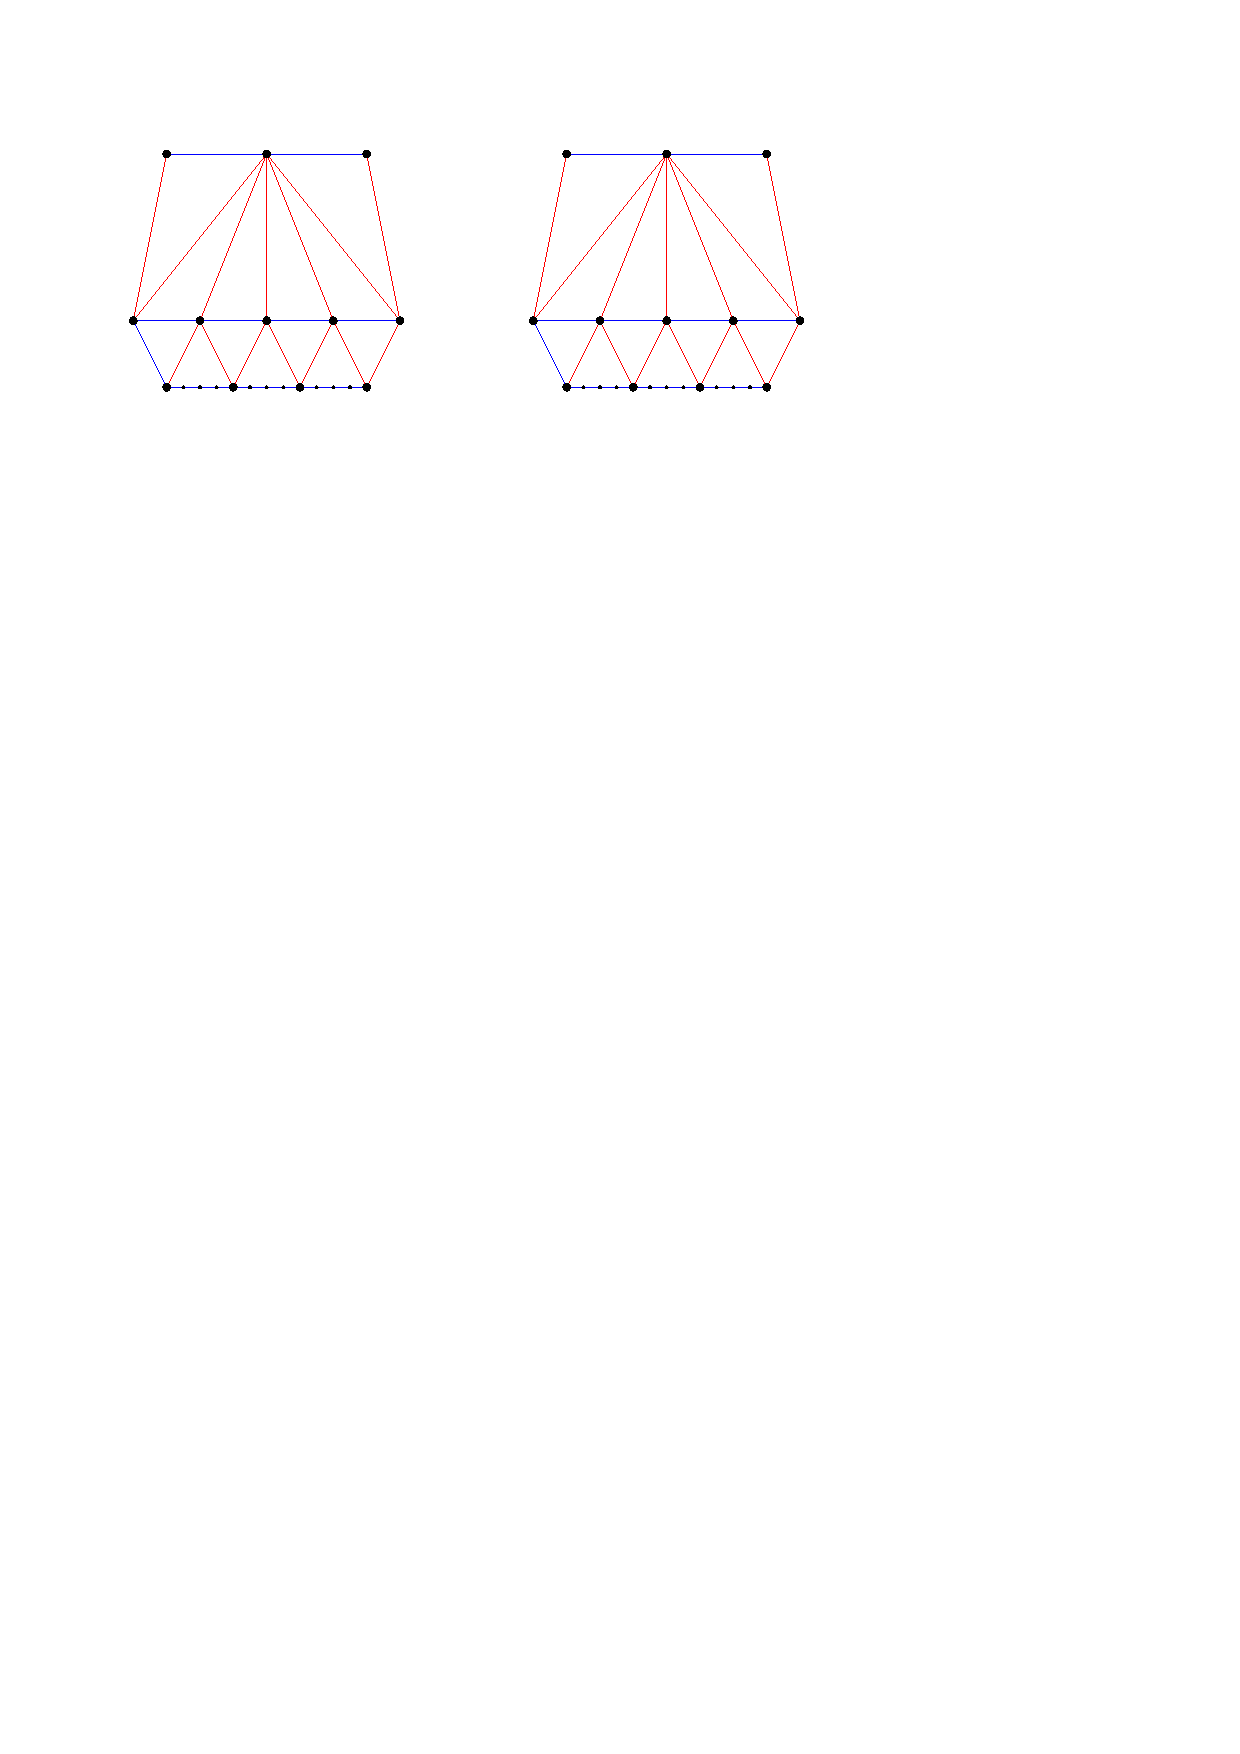
\includegraphics[width =\textwidth]{topFanFlips/img/splitfront}
        \caption{Trouble!}
        \label{fig:fanflip:splitFirstVertex}

    \end{subfigure}

    \caption{}
    \label{fig:fanflip:fanflips}
\end{figure}


\paragraph{Description}
When we encounter a topfan we start flipping edges.

We can just flip above a merge. So we do that.

We can't continue flipping above a join. So we don't so this. Instead we mark an edge for potential topload. We will see in the next section how we treat these edges in the next section.

\paragraph{What topfan flip do we do?}
We consider all faces we currently have in a topdown order. We don't consider topfans whose left edge is already blue. \fxnote{These topfans must be followed by a small botfan. But maybe we will still want to request a closing? Or we want to treat the last topfan below?}

A topfan is above a number of edges of the bottom fence. These edges are the rim of the fan.  Along this fan we can't have a merge followed by a split. Unless we are south adjacent (but we can solve this by splitting the fans). See the paragraph below.

This means the rim of a fan can have a number of merges followed by a number of splits.

If the rim has no merges or splits we execute the topfanflip depicted in Figure \ref{fig:fanflip:regular}. We color all but the rightmost fan edge blue, color all but the rightmost rim edge red. And color the left sides of all topfans below this topfan in the face below the current face blue.

If the rim consists of only merges we can easily adept a topfanflip to this situation. We simply don't flip the edge merging in as depicted in Figure \ref{fig:fanflip:merge}.

A special case is given by a merge on the last vertex on the bottom edges of the top fan. In that case we flip all rim edges (even the last one) to prevent a blue $Z$ from forming. See figure \ref{fig:fanflip:mergeLastVertex}.

Splits are more difficult to handle. We are unfortunatly unable to keep flipping once we hit a split hence we stop before we get that far. See Figure \ref{fig:fanflip:split}. It this happens on the first vefrtex we don't flip at all, see Figure \ref{fig:fanflip:splitFirstVertex}. In both cases we indicate a topload with a red $\ell$.


\paragraph{The result}
Befor the topfanflips we had a vertically one-sided REL. After we have a vertically onsided REL. With no large top-fans except at the beginning of faces. Except for the \emph{Trouble!} case.

\begin{lemma}
  \label{lm:}
  If the graph was onesided before a topfanflip it is still onesided after such a flip in the regular and merge cases.
\end{lemma}
\begin{proof}
  Let us first consider the regular case. Since the edge  $v_n w_m$ is red (otherwise we would have a merge) this change doesn't produce any blue $Z$'s.

  Let us also consider the other merge cases. Due to the   clever recoloring these also don't lead to a merge. However they can lead to a face starting with a large topfan. We will later see this is a controlled topfan.

  It is clear the split cases also don't produce a blue $Z$. But the topfans are again controlled. As we will see in the next section.
\end{proof}


\begin{lemma}
  \label{lm:}
  In the remaing faces every large topfan is in one of the following two situations.
  \begin{enumerate}
    \item  This topfan is at the start of the face
    \item  This topfan is followed by a botfan of size 2 followed by a topfan of unknown size.
  \end{enumerate}
\end{lemma}
\begin{proof}
  The first thing happens in the merge on the last vertex cases. The second thing happens in cases with a split.
\end{proof}


\paragraph{Topfans below topfans}
We in principle try to flip all topfans. We do this in a topdown manner.


\paragraph{South-adjacent topfans}
We call a topfan south-adjecent if any of it's rim vertices is next to the south pole.

At most two vertices of a top fan can be adjecent to the south pole. And in this case these vertices must be adjecent. Otherwise we have a seperating 4-cycle.

Before the south pole we can have a split followed by a merge followed by the south pole adjecent vertices followed again by possibly splits and merges.

Furtunatly we can treat this complicated faces just like any split fan. Where we stop flipping before the first split or $\pS$-adjacent vertex.



\paragraph{Trouble}
(If) we can't do anything with the \emph{Trouble!} case  it will increase our bound by $$\max_{(u,v) \in E}   \min\parens{ \deg(u), \deg(v) }$$

We can prove this bound by using  to well-placed chords. \fxnote{We might be able to prevent Trouble! with 3chords. But I'm not sure. I don't think it is straightforward. }

I'm going to ignore this for now.

I guess the other topload can also be very unfortunate. It can even be next to a very large split. So it runs in the same trouble as Trouble.

We kinda want only merges to a certain middle line and only joins afterwards. We can make that transition with topfans. We just can't transition back.

Something weird with topfans adjecent to $\pS$ view them as separate fans. Then things i say are true. Not entirily tough
